% !TeX program = xelatex
% Single LaTeX source. Keep trim.png beside this file when compiling.
\documentclass[a4paper,11pt]{article}
\usepackage[margin=22mm]{geometry}
\usepackage{amsmath,amssymb,bm,booktabs,longtable,array,graphicx,float}
\usepackage{pdflscape,tikz,listings,xcolor}
\usetikzlibrary{arrows.meta,positioning,calc}
\usepackage[colorlinks=true,linkcolor=blue!55!black,urlcolor=blue!55!black]{hyperref}
\setcounter{tocdepth}{2}
\setcounter{MaxMatrixCols}{12}
\setlength{\parskip}{0.35em}
\setlength{\emergencystretch}{2em}
\renewcommand{\arraystretch}{1.15}
\lstset{language=Matlab,basicstyle=\ttfamily\small,breaklines=true,
  columns=fullflexible,frame=single,showstringspaces=false,
  keywordstyle=\color{blue!60!black},commentstyle=\color{green!35!black}}
\newcommand{\dd}{\mathrm{d}}
\newcommand{\de}{\delta_e}
\newcommand{\dt}{\delta_T}
\newcommand{\Gq}{G_{q\delta_e}}
\newcommand{\file}[1]{\mbox{\texttt{\small\detokenize{#1}}}}
\title{AERO5560 Group 8\\Aircraft Modelling and Pitch-Rate Feedback\\\large Progress Report: Data, Trim, Linearisation and Inner-Loop Architecture}
\author{Group 8}
\date{19 October 2026}
\begin{document}
\maketitle
\begin{abstract}
This report documents the completed extraction of Group 8 aircraft data, trim verification, numerical linearisation, and the elevator-to-pitch-rate transfer function, together with the construction and labelling of the pitch-rate feedback loop required by the assignment. The supplied initial condition, approximately 200 knots at 300 ft, satisfies numerical equilibrium and maintains its initial speed and attitude during a 60 s undisturbed nonlinear simulation. Five central-difference step sizes are used to obtain the full $12\times12$ state matrix $A$ and $12\times5$ input matrix $B$, followed by a fixed-altitude, four-state longitudinal model. The resulting $\Gq(s)$ has a zero at the origin and a ZPK gain of approximately $-88.196939$. The feedback architecture uses unity measurement and an ideal elevator actuator, with all command, error, control and output signals defined. Closed-loop and sensitivity--complementary-sensitivity--compensator (SCK) expressions are derived. The compensator $K_q(s)$ remains to be designed; no claim is made that the closed-loop performance specifications have been met.
\end{abstract}
\clearpage
\tableofcontents
\clearpage

\section{Scope and Modelling Conventions}
This stage addresses two requirements in Longitudinal Task 1: determining $\Gq$ for the assigned aircraft, and constructing a fully labelled feedback loop that controls pitch rate using the elevator. The preceding data extraction, trim verification and linearisation provide the model used for these requirements. The three compensator designs, outer loop, gust analysis, auto-throttle and complete autopilot integration remain subsequent tasks.

The full state vector contains body-axis velocities and angular rates, Euler attitude angles, and earth-frame positions:
\begin{equation}
\bm X=[u,v,w,p,q,r,\phi,\theta,\psi,X_e,Y_e,Z_e]^{\mathsf T}.
\end{equation}
The control-input vector is
\begin{equation}
\bm U=[\dt,\de,\delta_a,\delta_r,\delta_f]^{\mathsf T},
\end{equation}
representing throttle, elevator, aileron, rudder and flap, respectively. Internal calculations use SI units: m/s for velocity, m for position, rad for angles, rad/s for angular rates, and a $0$--$1$ throttle fraction. Altitude is $h=-Z_e$, and vertical speed is $V_s=-\dot Z_e$, positive upwards.

Linear-model variables are increments about the nominal flight trajectory:
\begin{equation}
\bm X=\bm X_{\rm ref}(t)+\Delta\bm X,\qquad
\bm U=\bm U_0+\Delta\bm U.
\end{equation}
Because the aircraft continues to move forward in earth coordinates, the $X_e$ component of $\bm X_{\rm ref}(t)$ is not constant. The position derivatives must not all be required to vanish, and an incremental control deflection must not be treated as an absolute deflection.

\section{Group 8 Aircraft Data}
The Group 8 function \file{FlightDataAircraft8.p} was executed in MATLAB R2025b Update 7. Initial conditions were loaded from \file{ICsAircraft8_200knts_300ft.mat}. These files provide the aircraft parameter structure and initial vectors. The data do not identify a real aircraft type or manufacturer; the model is therefore referred to as the Group 8 aircraft.

\subsection{Mass, Geometry and Propulsion}
\begin{table}[H]\centering
\caption{Principal aircraft parameters extracted from the supplied data}
\begin{tabular}{llr}\toprule
Parameter&Description&Value\\\midrule
$m$&Mass&750 kg\\
$g$&Gravitational acceleration&9.81 m/s$^2$\\
$S$&Reference wing area&11.9 m$^2$\\
$b$&Wingspan&7 m\\
$c$&Reference chord&0.85 m\\
$I_{xx}$&Roll moment of inertia&605.29 kg\,m$^2$\\
$I_{yy}$&Pitch moment of inertia&1766.52 kg\,m$^2$\\
$I_{zz}$&Yaw moment of inertia&2168.83 kg\,m$^2$\\
$I_{xz}$&Product-of-inertia parameter&84.71 kg\,m$^2$\\
$P_{\max}$&Maximum power parameter&253.504 kW\\
$\eta$&Propeller efficiency parameter&0.85\\\bottomrule
\end{tabular}
\end{table}
The corresponding aspect ratio is $b^2/S=4.11765$, and wing loading is $mg/S=618.277\,\mathrm{N/m^2}$. The maximum power parameter is not the thrust at the trim condition.

The legacy fields are mapped to the names required by the current nonlinear simulation framework, as instructed in the data package:
\begin{lstlisting}
FlightData = FlightDataAircraft8();
FlightData.Geometric = FlightData.Geo;
FlightData.Inertial = FlightData.I;
FlightData.Propeller = FlightData.Prop;
\end{lstlisting}
\subsection{Initial State and Controls}
\begin{equation}
\begin{aligned}
\bm X_0={}&[102.8869153573,\;0,\;0.4724322704,\;0,\;0,\;0,\\
 &\phantom{[}0,\;0.004591730139,\;0,\;0,\;0,\;-91.44]^{\mathsf T},
\end{aligned}
\end{equation}
Each entry uses the units specified in the state-vector definition above.
\begin{equation}
\bm U_0=[0.7703166691,\;0.01337052176,\;0,\;0,\;0]^{\mathsf T}.
\end{equation}
The principal conditions are also listed in Table~\ref{tab:trimpoint} for clarity.
\begin{table}[H]\centering
\caption{Initial flight condition and controls}\label{tab:trimpoint}
\begin{tabular}{lr}\toprule
Quantity&Value\\\midrule
$V_0=\sqrt{u_0^2+v_0^2+w_0^2}$&102.888 m/s, approximately 199.99827 knots\\
$h_0=-Z_{e0}$&91.44 m, 300 ft\\
$\alpha_0=\operatorname{atan2}(w_0,u_0)$&$0.263086758^\circ$\\
$\theta_0$&$0.263086758^\circ$\\
$\beta_0,\phi_0,\psi_0$&$0$\\
$p_0,q_0,r_0$&$0$\\
Throttle&$77.0316669\%$\\
Elevator&$+0.766074467^\circ$\\
Aileron, rudder and flap&$0^\circ$\\\bottomrule
\end{tabular}
\end{table}

The body-axis velocity $w_0=0.4724322704$ m/s does not imply a climb. Earth-frame vertical speed is
\begin{equation}\label{eq:vs}
V_s=u\sin\theta-v\sin\phi\cos\theta-w\cos\phi\cos\theta.
\end{equation}
Substituting the Group 8 initial condition gives $V_{s0}=0$, consistent with level flight and $\theta_0=\alpha_0$.

\subsection{Control Limits}
The supplied data specify a throttle range of $[0,1]$ and elevator, aileron and rudder limits of $\pm25^\circ$. The assignment explicitly limits the aileron to $\pm20^\circ$; the stricter assignment limit must be used for lateral performance assessment. No flap-deflection or control-rate limits are provided in these data.

The pitch-rate inner loop must respect the absolute elevator limit:
\begin{equation}\label{eq:limit}
-25^\circ\leq\delta_{e0}+\Delta\de(t)\leq25^\circ.
\end{equation}
Since $\delta_{e0}=0.766074467^\circ$, the available incremental elevator range is approximately
\[
[-25.766074467^\circ,\;24.233925533^\circ].
\]
The remaining positive throttle increment is $1-0.7703166691=0.2296833309$.

\section{Nonlinear Trim Verification}
\subsection{Method}
With zero gust and the original $\bm X_0,\bm U_0$, the supplied \file{aero5560_aero.p} and \file{aero5560_motion.p} functions are evaluated. Because the aerodynamic model depends on state derivatives, the following consistency iteration is required:
\begin{align}
(\bm C_F^{(k)},\bm C_M^{(k)})
 &=\mathcal A(\bm X_0,\bm 0,\dot{\bm X}^{(k)},\bm U_0,F),\\
\dot{\bm X}^{(k+1)}
 &=\mathcal M(\bm X_0,\bm C_F^{(k)},\bm C_M^{(k)},F).
\end{align}
The iteration terminates when the infinity norm of the update is below $10^{-11}$, with a maximum iteration count enforced. At the initial condition, convergence is obtained in two iterations, with a final update norm of zero.

\subsection{Residuals and Unforced Simulation}
\begin{table}[H]\centering
\caption{Initial state-derivative residuals}
\begin{tabular}{ll}\toprule
Quantity&Result\\\midrule
$\dot u$&$-2.4980\times10^{-16}$ m/s$^2$\\
$\dot v,\dot w$&$0$ m/s$^2$\\
$\dot p,\dot q,\dot r$&$0$ rad/s$^2$\\
$\dot\phi,\dot\theta,\dot\psi$&$0$ rad/s\\
$\dot X_e$&$102.888$ m/s, expected forward motion\\
$\dot Y_e,\dot Z_e$&$0$ m/s\\\bottomrule
\end{tabular}
\end{table}
The diagnostic tolerances chosen for this check are $10^{-4}$ m/s$^2$ for translational acceleration, $10^{-6}$ in the corresponding SI units for angular acceleration and attitude rates, and $10^{-4}$ m/s for lateral and vertical earth-frame velocities. These are engineering checks rather than assignment grading thresholds; the actual residuals are much smaller.

With $\bm U_0$ fixed and no gust or feedback, the full nonlinear model is integrated for 60 s using \texttt{ode45}. The first run uses relative tolerance $10^{-9}$, absolute tolerance $10^{-11}$ and maximum step 0.05 s. A tighter check uses $10^{-10}$, $10^{-12}$ and 0.025 s. Outputs are sampled every 0.1 s, yielding 601 points.

Both runs retain the initial speed, altitude, vertical speed, angle of attack, pitch angle and three angular rates. Differences in these outputs are zero in the saved double-precision results. The final forward position is $X_e(60)\approx6173.28$ m, consistent with $V_0t$. The supplied trim point can therefore be retained for linearisation. Figure~\ref{fig:trim} shows the computed histories.
\begin{figure}[H]\centering
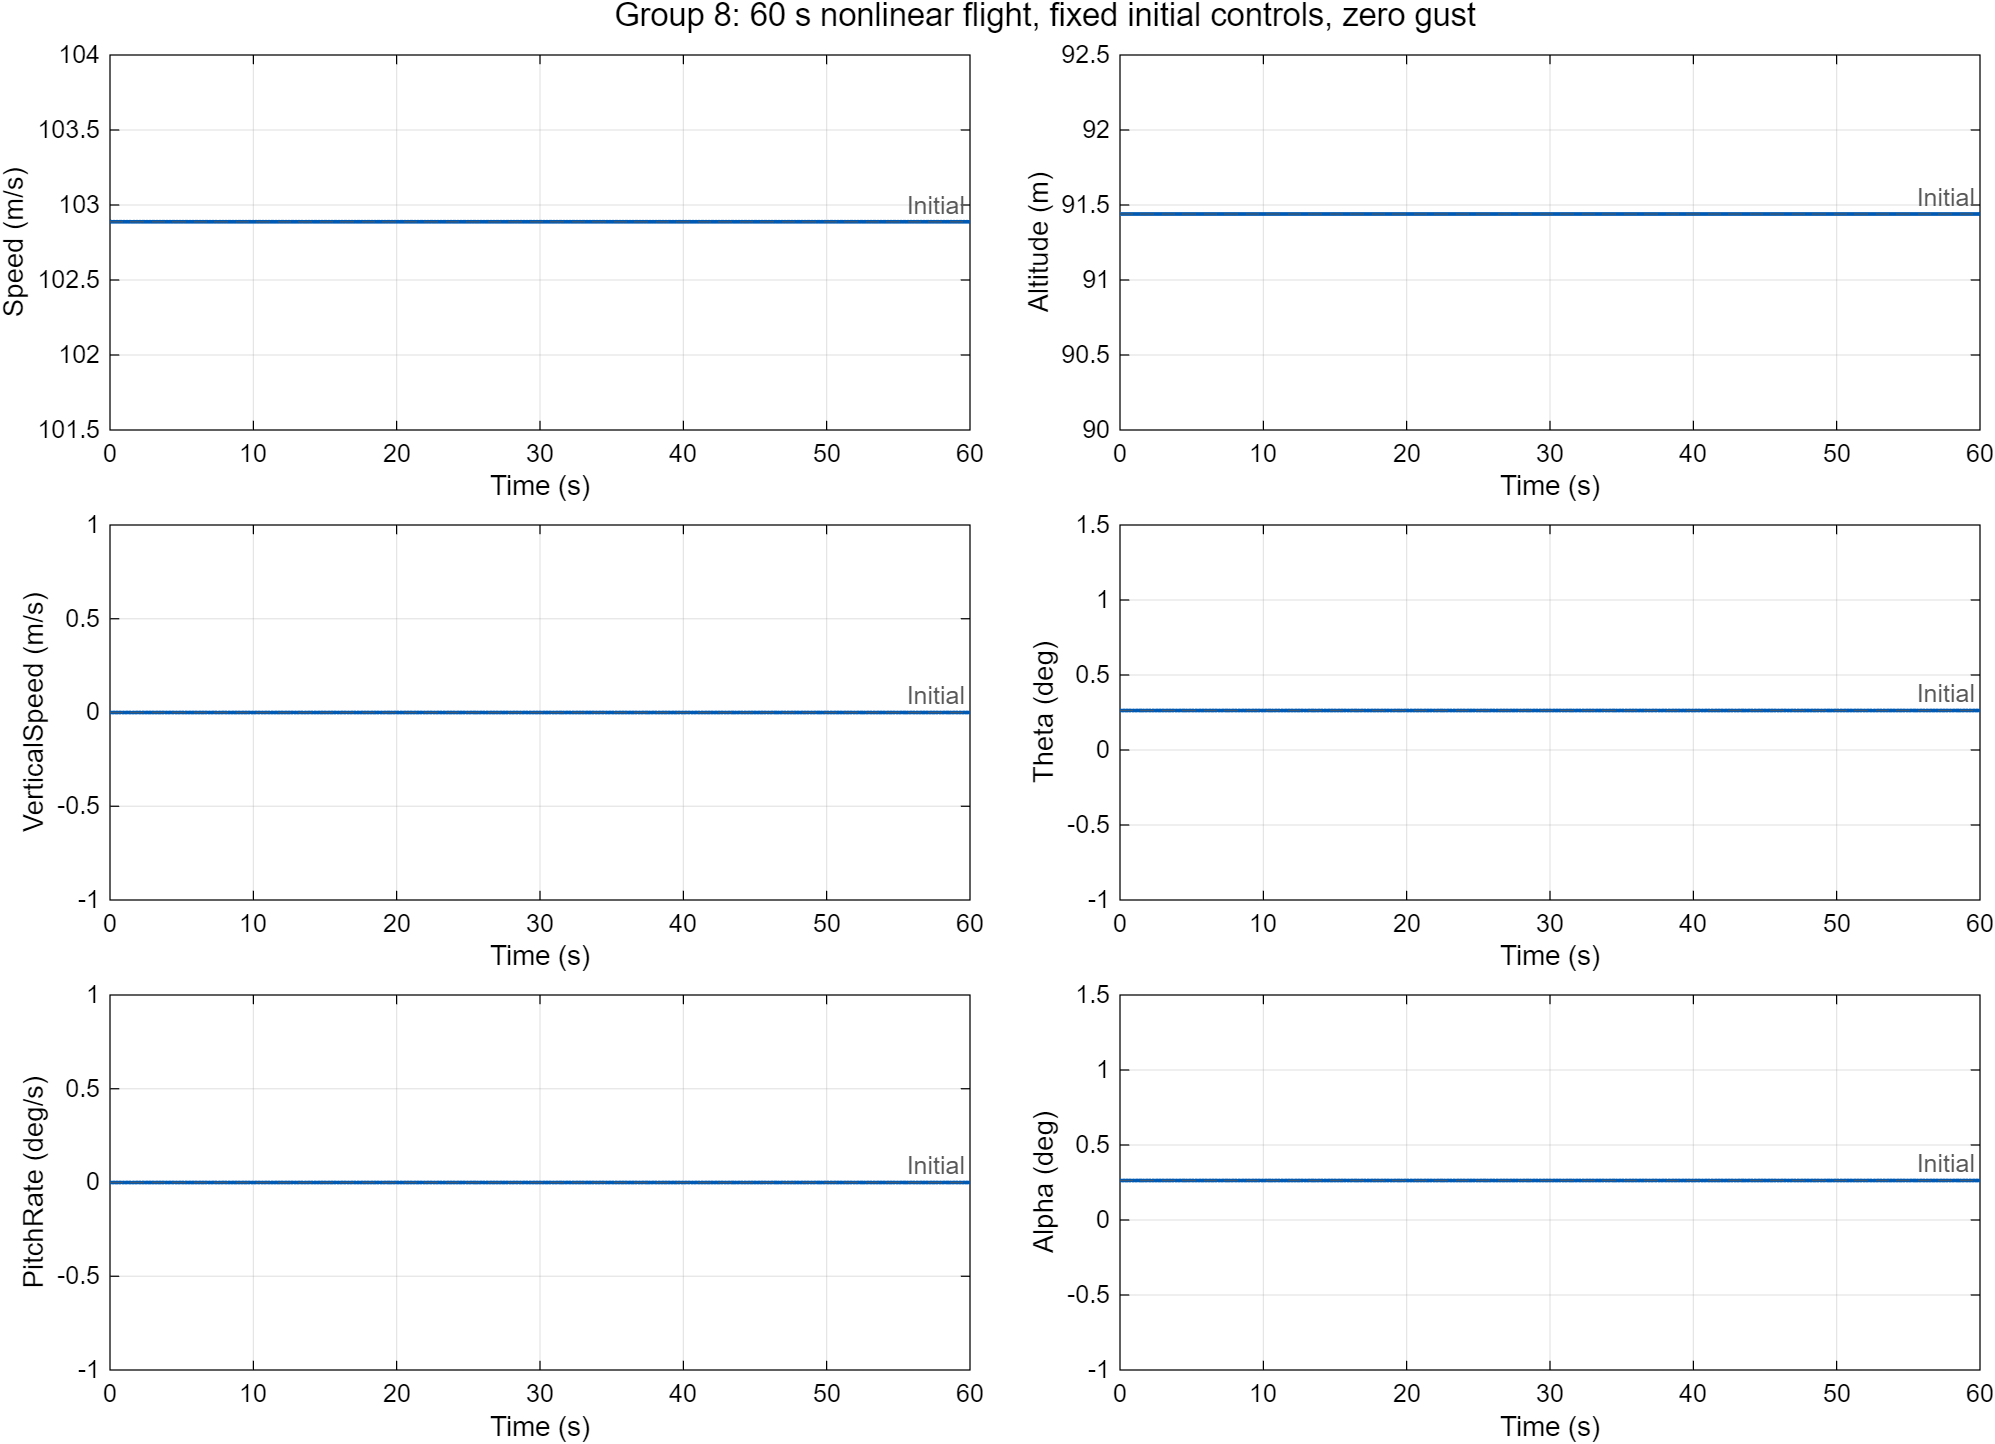
\includegraphics[width=0.94\linewidth]{trim.png}
\caption{A 60 s nonlinear simulation of Group 8 with fixed initial controls and zero gust.}\label{fig:trim}
\end{figure}
Remaining at an exact equilibrium without disturbance does not by itself prove disturbance stability. Stability must also be assessed using the linearised poles and perturbed responses.

\section{Numerical Linearisation and State-Space Models}
\subsection{Central Differences and Numerical Checks}
Near the nominal trim trajectory, the perturbation model is
\begin{equation}\label{eq:ss}
\Delta\dot{\bm X}=A\Delta\bm X+B\Delta\bm U.
\end{equation}
The Jacobian columns are calculated using central differences:
\begin{align}
A_{:,i}&\approx\frac{f(\bm X_0+h_i\bm e_i,\bm U_0)-f(\bm X_0-h_i\bm e_i,\bm U_0)}{2h_i},\\
B_{:,j}&\approx\frac{f(\bm X_0,\bm U_0+k_j\bm e_j)-f(\bm X_0,\bm U_0-k_j\bm e_j)}{2k_j}.
\end{align}
Every evaluation of $f$ reconverges the implicit state derivatives. State increments are scaled according to velocity, angle/angular-rate and position magnitudes; control scales are unity. Relative steps of $10^{-4},3\times10^{-5},10^{-5},3\times10^{-6},10^{-6}$ are compared, and the middle value, $10^{-5}$, is selected.

\begin{table}[H]\centering
\caption{Relative Frobenius-norm differences from the selected Jacobians}
\begin{tabular}{rrr}\toprule
Relative step&$\|A_h-A\|_F/\|A\|_F$&$\|B_h-B\|_F/\|B\|_F$\\\midrule
$10^{-4}$&$1.1803\times10^{-9}$&$5.1592\times10^{-12}$\\
$3\times10^{-5}$&$9.5524\times10^{-11}$&$5.5809\times10^{-13}$\\
$10^{-5}$&$0$&$0$\\
$3\times10^{-6}$&$1.1302\times10^{-11}$&$1.6652\times10^{-11}$\\
$10^{-6}$&$2.3360\times10^{-10}$&$9.7214\times10^{-11}$\\\bottomrule
\end{tabular}
\end{table}
An independent mixed-perturbation Taylor check gives residuals of approximately $5.2498\times10^{-5}$, $1.3124\times10^{-5}$ and $3.2808\times10^{-6}$ as the perturbation amplitude is successively halved. The error ratios, 4.0002 and 4.0001, agree with the quadratic remainder expected from first-order linearisation. Agreement in a global norm does not imply identical relative accuracy for individual near-zero entries.

\subsection{Four-State Longitudinal Model}
Under the fixed-altitude approximation, state indices $[1,3,5,8]$ and input indices $[1,2]$ give
\begin{equation}
\bm x_\ell=[\Delta u,\Delta w,\Delta q,\Delta\theta]^{\mathsf T},\qquad
\bm u_\ell=[\Delta\dt,\Delta\de]^{\mathsf T}.
\end{equation}
\begin{equation}\label{eq:alon}
A_\ell=\begin{bmatrix}
-0.06144334&0.05552868&-0.47243227&-9.80989658\\
-0.16960655&-4.78731236&99.44823052&-0.04504471\\
0.0002475794&-0.11258862&-3.67476184&0\\
0&0&1&0
\end{bmatrix},
\end{equation}
\begin{equation}\label{eq:blon}
B_\ell=\begin{bmatrix}
2.76318036&0\\
-5.9699623\times10^{-5}&-62.90658081\\
-1.7950804\times10^{-5}&-88.19693912\\
0&0
\end{bmatrix}.
\end{equation}
The second state is body-axis velocity $w$, not angle of attack $\alpha$. Changing to an angle-of-attack state requires a consistent transformation of both matrices.

The four-state longitudinal eigenvalues are
\begin{equation}
\lambda_{\rm SP}=-4.2313617\pm3.3004001\mathrm i,\qquad
\lambda_{\rm ph}=-0.03039711\pm0.07729208\mathrm i.
\end{equation}
These represent the short-period and phugoid modes, respectively, and lie in the left half-plane.

\subsection{Altitude and Lateral-Directional Models}
The $Z_e$ column of the full $A$ matrix contains nonzero terms. A five-state longitudinal model retaining altitude uses $[u,w,q,\theta,Z_e]$ and has also been saved. The four-state approximation omits altitude feedback. This report extracts $\Gq$ from Eqs.~\eqref{eq:alon}--\eqref{eq:blon}, consistently using the four-state model.

The lateral-directional states are $[v,p,r,\phi,\psi]$, with aileron and rudder inputs. Their poles are approximately $-13.81679$, $-0.719193\pm2.625197\mathrm i$, $-0.0119723$, and a zero heading-integrator pole. Position/heading zero eigenvalues in the full model do not imply divergent dynamics, but neither do they establish asymptotic return of all position states to the origin. Full and additional subsystem matrices are provided in the appendices.

\subsection{Small-Step Linear and Nonlinear Comparisons}
The full 12-state $A,B$ model is compared with the nonlinear model for a $+0.05^\circ$ elevator increment and a $+0.001$ throttle increment over 10 s. The linear response is computed using matrix exponentials and the nonlinear response using \texttt{ode45}. Outputs are airspeed, $q$, and the vertical speed defined in Eq.~\eqref{eq:vs}.
\begin{table}[H]\centering
\caption{Maximum absolute output errors over the 10 s comparisons}
\begin{tabular}{lrrr}\toprule
Input step&Speed (m/s)&$q$ ($^\circ$/s)&$V_s$ (m/s)\\\midrule
Elevator increment&0.016588&0.023974&0.641690\\
Throttle increment&$2.0867\times10^{-6}$&$1.3892\times10^{-7}$&$2.5237\times10^{-7}$\\\bottomrule
\end{tabular}
\end{table}
For the elevator test, the maximum $V_s$ error during the first 2 s is approximately 0.004968 m/s, or 0.2253\% of the nonlinear peak over that interval. By 10 s, however, the vertical-speed peak is approximately 11.93 m/s and the speed change is approximately 4.69 m/s. The aircraft has departed appreciably from the initial point, and the relative $V_s$ error grows to approximately 5.38\%. The comparison supports local agreement; sustained-input motion of this magnitude should not be treated as an infinitesimal perturbation.

\section{Elevator-to-Pitch-Rate Transfer Function}
\subsection{Output Selection and Derivation}
The second longitudinal input column corresponds to the elevator. Set
\begin{equation}
\begin{aligned}
B_q&=B_\ell(:,2)=\begin{bmatrix}0&-62.90658081&-88.19693912&0\end{bmatrix}^{\mathsf T},\\
C_q&=\begin{bmatrix}0&0&1&0\end{bmatrix},\qquad D_q=0.
\end{aligned}
\end{equation}
Taking the Laplace transform with zero initial perturbations gives
\begin{align}
s\Delta\bm x_\ell&=A_\ell\Delta\bm x_\ell+B_q\Delta\de,\\
\Delta q&=C_q\Delta\bm x_\ell,
\end{align}
and hence
\begin{equation}\label{eq:gdefinition}
\boxed{\Gq(s)=\frac{\Delta q(s)}{\Delta\de(s)}=C_q(sI-A_\ell)^{-1}B_q.}
\end{equation}
Here $C_q$ denotes the state-space output matrix. The complementary sensitivity below is denoted $\mathcal C_q$ to avoid ambiguity.

\subsection{ZPK and Polynomial Forms}
The zero-pole-gain representation, with complex-conjugate pole factors combined into real quadratics, is
\begin{equation}\label{eq:gfactored}
\boxed{\Gq(s)=\frac{-88.19693912\,s(s+4.704978073)(s+0.06347365466)}
{(s^2+8.462723331s+28.79706207)(s^2+0.06079421306s+0.006898050455)}.}
\end{equation}
The corresponding polynomial form is
\begin{equation}
\Gq(s)=\frac{-88.19693912s^3-420.5628467s^2-26.33932382s}
{s^4+8.523517544s^3+29.31844472s^2+1.809071019s+0.1986435871}.
\end{equation}
The zeros are
\begin{equation}
z=0,\quad -4.704978073,\quad -0.06347365466.
\end{equation}
The poles are the longitudinal four-state eigenvalues given above, and the ZPK gain is $-88.19693912$.

\subsection{Numerical Verification and Interpretation}
Equation~\eqref{eq:gfactored} is compared with the state-space frequency response at 501 points from $10^{-4}$ to $10^4$ rad/s. The maximum relative error is approximately $1.78\times10^{-13}$. An independently formed Cayley--Hamilton/Markov polynomial gives a maximum relative frequency-response error of approximately $7.20\times10^{-9}$.

One raw numerical zero is approximately $+2.40\times10^{-16}$. The model satisfies $q=\dot\theta$, the fourth entry of $B_q$ is zero, and $A_\ell$ is nonsingular, so an exact zero at the origin is expected. After verifying this structure and the DC gain, only this floating-point residual is set to zero. The raw object is retained; no general pole-zero cancellation is applied.

Since $\Gq(0)=0$, pitch rate returns to zero following a constant elevator input in this stable open-loop model. The leading high-frequency term is approximately $-88.19694/s$, indicating a negative direct pitch-acceleration response to a positive elevator increment. This sign must be handled consistently in the feedback design.

\section{Pitch-Rate Feedback-Loop Construction}\label{sec:loop}
\subsection{Objective and Assumptions}
The inner-loop objective is to make the actual pitch-rate increment $\Delta q$ follow the command $\Delta q_c$ using the elevator. Unity measurement, $H_q(s)=1$, and an ideal actuator, $A_e(s)=1$, are assumed for the linear perturbation design. Physical deflection limits are checked using Eq.~\eqref{eq:limit} and enforced in the nonlinear implementation. Saturation is nonlinear and is not represented by a fixed LTI transfer function in this section.

The compensator is denoted $K_q(s)$. Its order and parameters will be selected through at least three subsequent design options. The block diagram below defines the architecture and all signals at this stage.

\begin{figure}[H]\centering
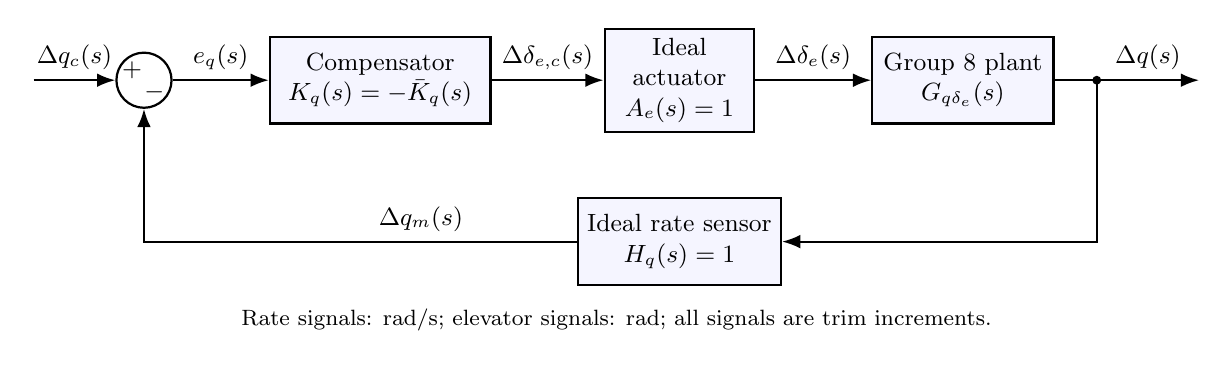
\begin{tikzpicture}[>=Latex,font=\small,
  block/.style={draw,thick,minimum height=1.1cm,align=center,fill=blue!4},
  every path/.style={thick}]
\node[circle,draw,minimum size=0.7cm,inner sep=0pt] (sum) at (1.2,0) {};
\node at ($(sum.center)+(-0.15,0.12)$) {$+$};
\node at ($(sum.center)+(0.13,-0.15)$) {$-$};
\node[block,minimum width=2.8cm] (K) at (4.2,0) {Compensator\\$K_q(s)=-\bar K_q(s)$};
\node[block,minimum width=1.9cm] (act) at (8.0,0) {Ideal\\actuator\\$A_e(s)=1$};
\node[block,minimum width=2.3cm] (plant) at (11.6,0) {Group 8 plant\\$\Gq(s)$};
\coordinate (take) at (13.3,0);
\node[block,minimum width=2.5cm] (sensor) at (8.0,-2.05) {Ideal rate sensor\\$H_q(s)=1$};
\draw[->] (-0.2,0) -- node[above] {$\Delta q_c(s)$} (sum.west);
\draw[->] (sum.east) -- node[above] {$e_q(s)$} (K.west);
\draw[->] (K.east) -- node[above] {$\Delta\delta_{e,c}(s)$} (act.west);
\draw[->] (act.east) -- node[above] {$\Delta\de(s)$} (plant.west);
\draw[->] (plant.east) -- (take) -- node[above] {$\Delta q(s)$} (14.6,0);
\fill (take) circle (1.6pt);
\draw[->] (take) |- (sensor.east);
\draw[->] (sensor.west) -| node[pos=0.18,above] {$\Delta q_m(s)$} (sum.south);
\node[align=center,font=\footnotesize] at (7.2,-3.05)
{Rate signals: rad/s; elevator signals: rad; all signals are trim increments.};
\end{tikzpicture}
\caption{Unity negative-feedback pitch-rate loop using the elevator. The controller includes the required sign; its parameters remain to be designed.}\label{fig:loop}
\end{figure}

\begin{table}[H]\centering
\caption{Signals and blocks in the pitch-rate feedback architecture}
\begin{tabular}{p{0.22\linewidth}p{0.56\linewidth}l}\toprule
Symbol&Definition&Units\\\midrule
$\Delta q_c$&Commanded pitch-rate increment&rad/s\\
$\Delta q_m$&Measured feedback, equal to $\Delta q$ for ideal measurement&rad/s\\
$e_q$&Command minus measured pitch rate&rad/s\\
$K_q(s)$&Signed compensator mapping pitch-rate error to elevator command&s\\
$\Delta\delta_{e,c}$&Commanded elevator-deflection increment&rad\\
$A_e(s)=1$&Ideal actuator: actual increment equals command&Dimensionless\\
$\Delta\de$&Actual elevator increment applied to the aircraft model&rad\\
$\Gq(s)$&Open-loop aircraft dynamics from elevator increment to $q$&$(\mathrm{rad/s})/\mathrm{rad}$\\
$\Delta q$&Actual pitch-rate increment&rad/s\\
$H_q(s)=1$&Unity pitch-rate measurement feedback&Dimensionless\\\bottomrule
\end{tabular}
\end{table}

\subsection{Feedback Sign and Operation}
The summing junction implements
\begin{equation}\label{eq:error}
e_q=\Delta q_c-\Delta q_m.
\end{equation}
A command above the actual pitch rate produces positive error. In this aircraft model, a positive elevator increment has a negative direct effect on $q$, so the controller must generate an appropriate negative elevator action. The sign is retained within the compensator by writing $K_q=-\bar K_q$. This is a sign convention, not a stability proof. Root-locus, frequency-domain and closed-loop pole checks remain necessary; a minus sign at the summing junction alone does not establish stability.

The signal relationships are
\begin{align}
\Delta\delta_{e,c}&=K_q e_q,\\
\Delta\de&=A_e\Delta\delta_{e,c},\\
\Delta q&=\Gq\Delta\de,\\
\Delta q_m&=H_q\Delta q.
\end{align}
For example, a $4^\circ$/s command corresponds to $\Delta q_c=4\pi/180\approx0.06981317$ rad/s. The comparator, controller and aircraft model all use radians internally to avoid an unintended $180/\pi$ scaling factor.

\subsection{Closed-Loop Derivation and SCK Expressions}
Define the signed loop transfer function as
\begin{equation}
L_q=K_q A_e\Gq H_q.
\end{equation}
Combining Eq.~\eqref{eq:error} with the forward-path relationships gives
\begin{equation}
\Delta q=\Gq A_eK_q(\Delta q_c-H_q\Delta q),
\end{equation}
Thus the general closed-loop relationships are
\begin{equation}
\frac{\Delta q}{\Delta q_c}=\frac{\Gq A_eK_q}{1+L_q},\qquad
\frac{\Delta\de}{\Delta q_c}=\frac{A_eK_q}{1+L_q}.
\end{equation}
For the assumptions $A_e=H_q=1$, define sensitivity and complementary sensitivity by
\begin{equation}\label{eq:sck}
S_q=\frac{1}{1+\Gq K_q},\qquad
\mathcal C_q=\frac{\Gq K_q}{1+\Gq K_q},\qquad S_q+\mathcal C_q=1.
\end{equation}
The resulting SCK relationships are
\begin{equation}\label{eq:cl}
\boxed{\frac{\Delta q}{\Delta q_c}=\mathcal C_q,\quad
\frac{e_q}{\Delta q_c}=S_q,\quad
\frac{\Delta\de}{\Delta q_c}=K_qS_q.}
\end{equation}
The complementary sensitivity $\mathcal C_q$ describes command tracking, $S_q$ describes tracking error and responses at appropriate disturbance locations, and $K_qS_q$ gives elevator demand. No noise or gust input is silently introduced at an unspecified point. Subsequent gust transfer functions must be derived for their actual injection locations.

Let $N_G,D_G$ be the numerator and denominator in Eq.~\eqref{eq:gfactored}, and write $K_q=N_K/D_K$. The closed-loop characteristic equation is
\begin{equation}
D_GD_K+N_GN_K=0.
\end{equation}
The numerator $N_K$ already includes the controller sign. When using $K_q=-\bar K_q$, the minus sign must not be duplicated or omitted elsewhere. Once the compensator is selected, these relationships provide the numerical closed-loop ZPK forms. Symbolic relationships are retained at this stage.

\subsection{Trim Bias and MATLAB Construction}
The linear loop produces the incremental elevator signal $\Delta\de$. For the nonlinear aircraft, the absolute input is
\begin{equation}
\de(t)=0.01337052176+\Delta\de(t)\quad(\mathrm{rad}),
\end{equation}
and must satisfy the absolute deflection limits. The ideal actuator in the linear diagram does not automatically implement saturation.

Once $K_q$ has been supplied by the subsequent design process, the same feedback structure can be constructed in MATLAB:
\begin{lstlisting}
load('Gqde.mat', 'Gqde');
% Kq must contain the intended controller sign.
Lq = Gqde * Kq;
Sq = feedback(1, Lq);       % error / q_command
Cq_closed = feedback(Lq,1); % q / q_command
Uq = feedback(Kq,Gqde);     % elevator_increment / q_command
% q_command = deg2rad(4);    % subsequent performance test
\end{lstlisting}
An equivalent function is provided in \file{loop.m}. The caller must supply the selected, signed $K_q$; the function does not choose an arbitrary controller or imply that performance specifications are met.

\section{Specifications for Subsequent Compensator Design}
The next stage compares at least three compensator designs using a $4^\circ$/s pitch-rate command. The assignment specifies a settling time of 3 s, steady-state error below 1\%, maximum overshoot below 20\%, and elevator deflection within its limits. It also gives a 2--10 rad/s frequency target and a noise bandwidth of 20 rad/s.

The assignment associates crossover frequency with a $-3$ dB point. Open-loop 0 dB gain crossover and closed-loop $-3$ dB bandwidth are generally different quantities and should be reported separately. The rise-time convention in Lecture 8-2 also differs from MATLAB's common 10--90\% default; the chosen definition must be stated.

Each design should document the compensator ZPK form, root locus, Bode plot, step response, elevator activity and a specification comparison table. The plant and feedback architecture are established here, but closed-loop compliance has not yet been demonstrated.

\section{Files, Reproduction and Sources}
\begin{table}[H]\centering
\caption{Current project scripts and outputs}
\begin{tabular}{p{0.25\linewidth}p{0.65\linewidth}}\toprule
Directory or entry point&Purpose\\\midrule
\file{trim/run_trim.m}&Trim residuals, 60 s unforced simulation and integration check\\
\file{linear/run_linear.m}&Central-difference A/B, subsystems, eigenvalues and local validation\\
\file{Gqde/run_Gqde.m}&Extraction of the Group 8 $\Gq$ and frequency-response verification\\
\file{AI_draft/loop.m}&Feedback transfer relationships for a supplied signed compensator\\
\file{AI_draft/report_en.tex}&Single English LaTeX source, including a native TikZ block diagram\\
\file{AI_draft/trim.png}&Figure exported from the actual trim simulation\\\bottomrule
\end{tabular}
\end{table}
Printed matrices and coefficients are rounded. Further numerical work should use the full-precision MAT/JSON files. This English backup preserves the technical content of the Chinese progress report and can support the modelling and inner-loop architecture sections of the final assignment report.

\begin{thebibliography}{9}
\bibitem{brief} AERO5560, \emph{Group Project: Aircraft Closed-Loop Control System Design and Analysis}, assignment brief, pp.~1--5.
\bibitem{data} \emph{Group8 AircraftData}: \file{FlightDataAircraft8.p}, \file{ICsAircraft8_200knts_300ft.mat}, and \file{Note.txt}.
\bibitem{framework} AERO5560, \emph{Flight Simulation Student Version}, supplied nonlinear functions and interface documentation.
\bibitem{lectures} AERO5560, Lectures 1-2, 2-1/2, 7-2, 8-1/2, 9-1/2 and 10-1: linearisation, transfer functions, feedback architectures and controller design.
\end{thebibliography}

\appendix
\clearpage
\begin{landscape}
\thispagestyle{plain}
\section{Full Twelve-State Matrices}
State and input ordering follows Section~1. The matrices below retain approximately eight significant figures. Each element has units given by its row's state-derivative units divided by its column-variable units.
\begin{center}\setlength{\arraycolsep}{3pt}\resizebox{\linewidth}{!}{$A=\begin{bmatrix}
-0.061443341 & 0 & 0.05552868 & 0 & -0.47243227 & 0 & 0 & -9.8098966 & 0 & 0 & 0 & 3.1754685\times10^{-5} \\
0 & -0.37729298 & 0 & 0.53108604 & 0 & -102.86881 & 9.8487485 & 0 & 0 & 0 & 0 & 0 \\
-0.16960655 & 0 & -4.7873124 & 0 & 99.448231 & 0 & 0 & -0.045044714 & 0 & 0 & 0 & -0.00094886847 \\
0 & -0.20268929 & 0 & -13.808594 & 0 & 1.4524332 & 0.019116101 & 0 & 0 & 0 & 0 & 0 \\
0.00024757942 & 0 & -0.11258862 & 0 & -3.6747618 & 0 & 0 & 0 & 0 & 0 & 0 & -1.3364074\times10^{-6} \\
0 & 0.058710969 & 0 & -0.54309133 & 0 & -1.0812624 & -0.0033528581 & 0 & 0 & 0 & 0 & 0 \\
0 & 0 & 0 & 1 & 0 & 0.0045917624 & 0 & 0 & 0 & 0 & 0 & 0 \\
0 & 0 & 0 & 0 & 1 & 0 & 0 & 0 & 0 & 0 & 0 & 0 \\
0 & 0 & 0 & 0 & 0 & 1.0000105 & 0 & 0 & 0 & 0 & 0 & 0 \\
0.99998946 & 0 & 0.004591714 & 0 & 0 & 0 & 0 & 0 & 0 & 0 & 0 & 0 \\
0 & 1 & 0 & 0 & 0 & 0 & -0.47243227 & 0 & 102.888 & 0 & 0 & 0 \\
-0.004591714 & 0 & 0.99998946 & 0 & 0 & 0 & 0 & -102.888 & 0 & 0 & 0 & 0 \\
\end{bmatrix}$}\end{center}
\end{landscape}
\clearpage
\subsection{Full Input Matrix}\begin{equation}B=\begin{bmatrix}
2.7631804 & 0 & 0 & 0 & 0 \\
0 & 0 & 3.7014393 & 20.777334 & 0 \\
-5.9699623\times10^{-5} & -62.906581 & 0 & 0 & 0 \\
0 & 0 & -318.33488 & -3.5101752 & 0 \\
-1.7950804\times10^{-5} & -88.196939 & 0 & 0 & 0 \\
0 & 0 & -16.168938 & -27.867108 & 0 \\
0 & 0 & 0 & 0 & 0 \\
0 & 0 & 0 & 0 & 0 \\
0 & 0 & 0 & 0 & 0 \\
0 & 0 & 0 & 0 & 0 \\
0 & 0 & 0 & 0 & 0 \\
0 & 0 & 0 & 0 & 0 \\
\end{bmatrix}\end{equation}

\section{Additional Subsystem Matrices}
\subsection{Five-State Longitudinal Model with Altitude}
States: $[u,w,q,\theta,Z_e]$; inputs: $[\dt,\de]$.
\begin{equation}\resizebox{0.95\linewidth}{!}{$A_{\ell,5}=\begin{bmatrix}
-0.061443341 & 0.05552868 & -0.47243227 & -9.8098966 & 3.1754685\times10^{-5} \\
-0.16960655 & -4.7873124 & 99.448231 & -0.045044714 & -0.00094886847 \\
0.00024757942 & -0.11258862 & -3.6747618 & 0 & -1.3364074\times10^{-6} \\
0 & 0 & 1 & 0 & 0 \\
-0.004591714 & 0.99998946 & 0 & -102.888 & 0 \\
\end{bmatrix}$}\end{equation}
\begin{equation}B_{\ell,5}=\begin{bmatrix}
2.7631804 & 0 \\
-5.9699623\times10^{-5} & -62.906581 \\
-1.7950804\times10^{-5} & -88.196939 \\
0 & 0 \\
0 & 0 \\
\end{bmatrix}\end{equation}
\subsection{Five-State Lateral-Directional Model}
States: $[v,p,r,\phi,\psi]$; inputs: $[\delta_a,\delta_r]$.
\begin{equation}\resizebox{0.95\linewidth}{!}{$A_{\rm lat}=\begin{bmatrix}
-0.37729298 & 0.53108604 & -102.86881 & 9.8487485 & 0 \\
-0.20268929 & -13.808594 & 1.4524332 & 0.019116101 & 0 \\
0.058710969 & -0.54309133 & -1.0812624 & -0.0033528581 & 0 \\
0 & 1 & 0.0045917624 & 0 & 0 \\
0 & 0 & 1.0000105 & 0 & 0 \\
\end{bmatrix}$}\end{equation}
\begin{equation}B_{\rm lat}=\begin{bmatrix}
3.7014393 & 20.777334 \\
-318.33488 & -3.5101752 \\
-16.168938 & -27.867108 \\
0 & 0 \\
0 & 0 \\
\end{bmatrix}\end{equation}

\clearpage
\section{Complete Extracted Aerodynamic Parameters}
Original parameter-field names are retained. Angle, angular-rate and rate-of-change derivatives may use nondimensional variables within the aerodynamic model and must not be inserted directly as dimensional A/B entries.
\begingroup\small\renewcommand{\arraystretch}{1.05}
\begin{table}[H]\centering\caption{Original Group 8 aerodynamic fields}\label{tab:aero}
\begin{tabular}{lrlr}\toprule Field&Value&Field&Value\\\midrule
\file{alpha_o} & $-0.013772917$ & \file{Cmad} & $0.9531$ \\
\file{Cdo} & $0.020342$ & \file{Cmde} & $-2.3941614$ \\
\file{k} & $0.063776$ & \file{Cnb} & $0.027705$ \\
\file{CLa} & $4.786$ & \file{Cnbd} & $-0.0051$ \\
\file{CLq} & $9.269$ & \file{Cnp} & $-0.000421$ \\
\file{CLad} & $-1.1439$ & \file{Cnr} & $-0.140618$ \\
\file{CLde} & $0.61398157$ & \file{Cnda} & $-0.015126086$ \\
\file{CLo} & $0.065917179$ & \file{Cndr} & $-0.11229973$ \\
\file{Cyb} & $-0.379162$ & \file{Clb} & $-0.024446$ \\
\file{Cybd} & $0.117$ & \file{Clbd} & $0.0068$ \\
\file{Cyp} & $0.016304$ & \file{Clp} & $-0.456441$ \\
\file{Cyr} & $0.1222$ & \file{Clr} & $0.0601$ \\
\file{Cyda} & $0.036153637$ & \file{Clda} & $-0.35735378$ \\
\file{Cydr} & $0.20294165$ & \file{Cldr} & $0.000394$ \\
\file{Cmo} & $0.03337$ & \file{CDdf} & $0$ \\
\file{Cma} & $-0.295926$ & \file{CLdf} & $0$ \\
\file{Cmq} & $-25.094866$ & \file{Cmdf} & $0$ \\
\bottomrule\end{tabular}\end{table}\endgroup
\end{document}
